\clearpage{\pagestyle{empty}\cleardoublepage}
\chapter{Gli impianti fotovoltaici e il loro monitoraggio}
%
L'\emph{effetto fotovoltaico} consiste nel passaggio di elettroni 
dalla \emph{banda di valenza} alla \emph{banda di conduzione} di 
un materiale, a causa dell'assorbimento di \emph{fotoni}. 
%
Tale fenomeno viene replicato all'interno dei \emph{moduli (o celle) 
fotovoltaici}, allo scopo di trasformare l'energia contenuta nella 
radiazione solare in energia elettrica.
%

%
I moduli fotovoltaici sono costituiti da materiali \emph{semiconduttori}, 
caratterizzati dall'avere un \emph{band gap} di dimensioni tali 
per cui \Item{i} gli elettroni riescono a passare dalla 
banda di valenza a quella di conduzione a seguito dell'apporto 
energetico fornito dalla radiazione solare,
\Item{ii} gli elettroni che effettuano il passaggio nella banda 
di conduzione non vengono neutralizzati.
%
\begin{figure}[!h]
\centering
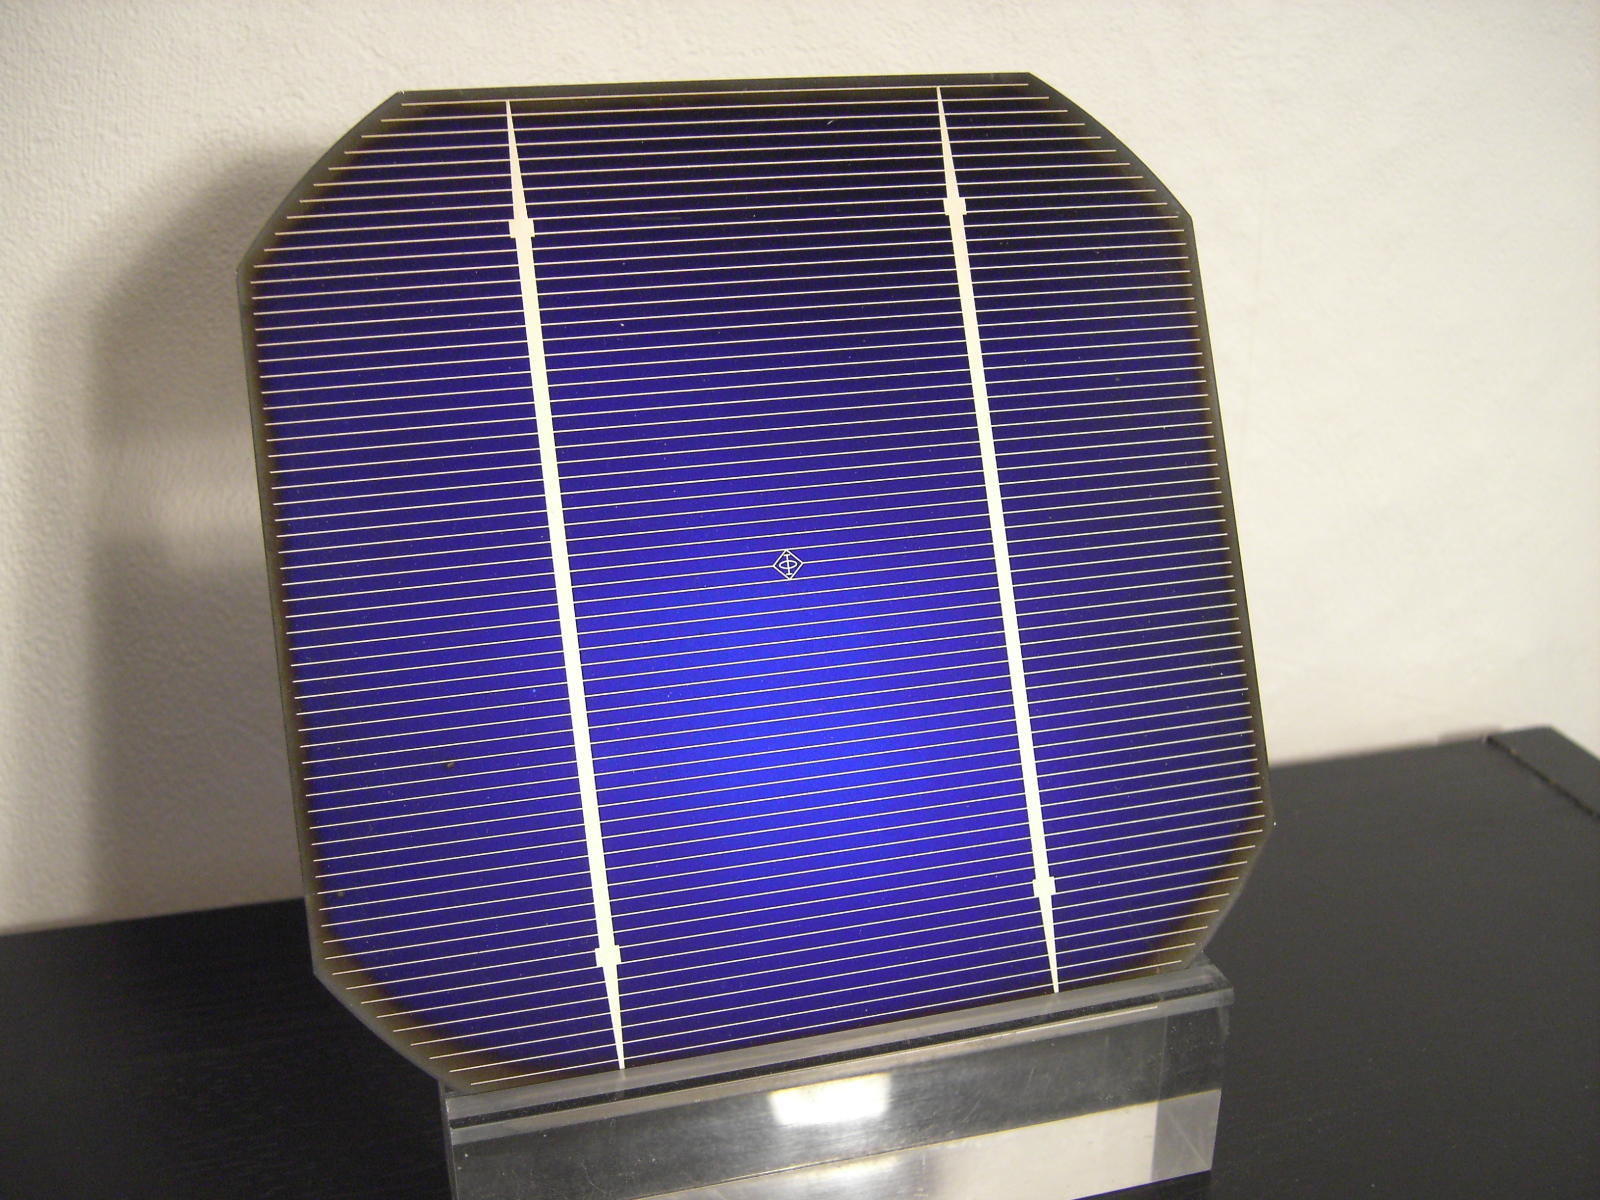
\includegraphics[width=350pt]{img/modulo-fotovoltaico.jpg}
\caption{Modulo fotovoltaico in silicio \emph{monocristallino}}
\end{figure}
%
Allo stato attuale, esistono diverse tecnologie di realizzazione di 
moduli fotovoltaici, la maggior parte delle quali prevedono l'utilizzo 
del silicio.








%% architettura tipica di un impianto fotovoltaico
%% quali informazioni si vogliono produrre?
%% quali informazioni e` necessario rilevare?
%% lista dei desiderata per un sistema di monitoraggio
